\documentclass{standalone}
\usepackage{tikz}
\usetikzlibrary{patterns, positioning}
\usepackage[sfdefault]{ClearSans} %% option 'sfdefault' activates Clear Sans as the default text font
\usepackage[T1]{fontenc}

\begin{document}
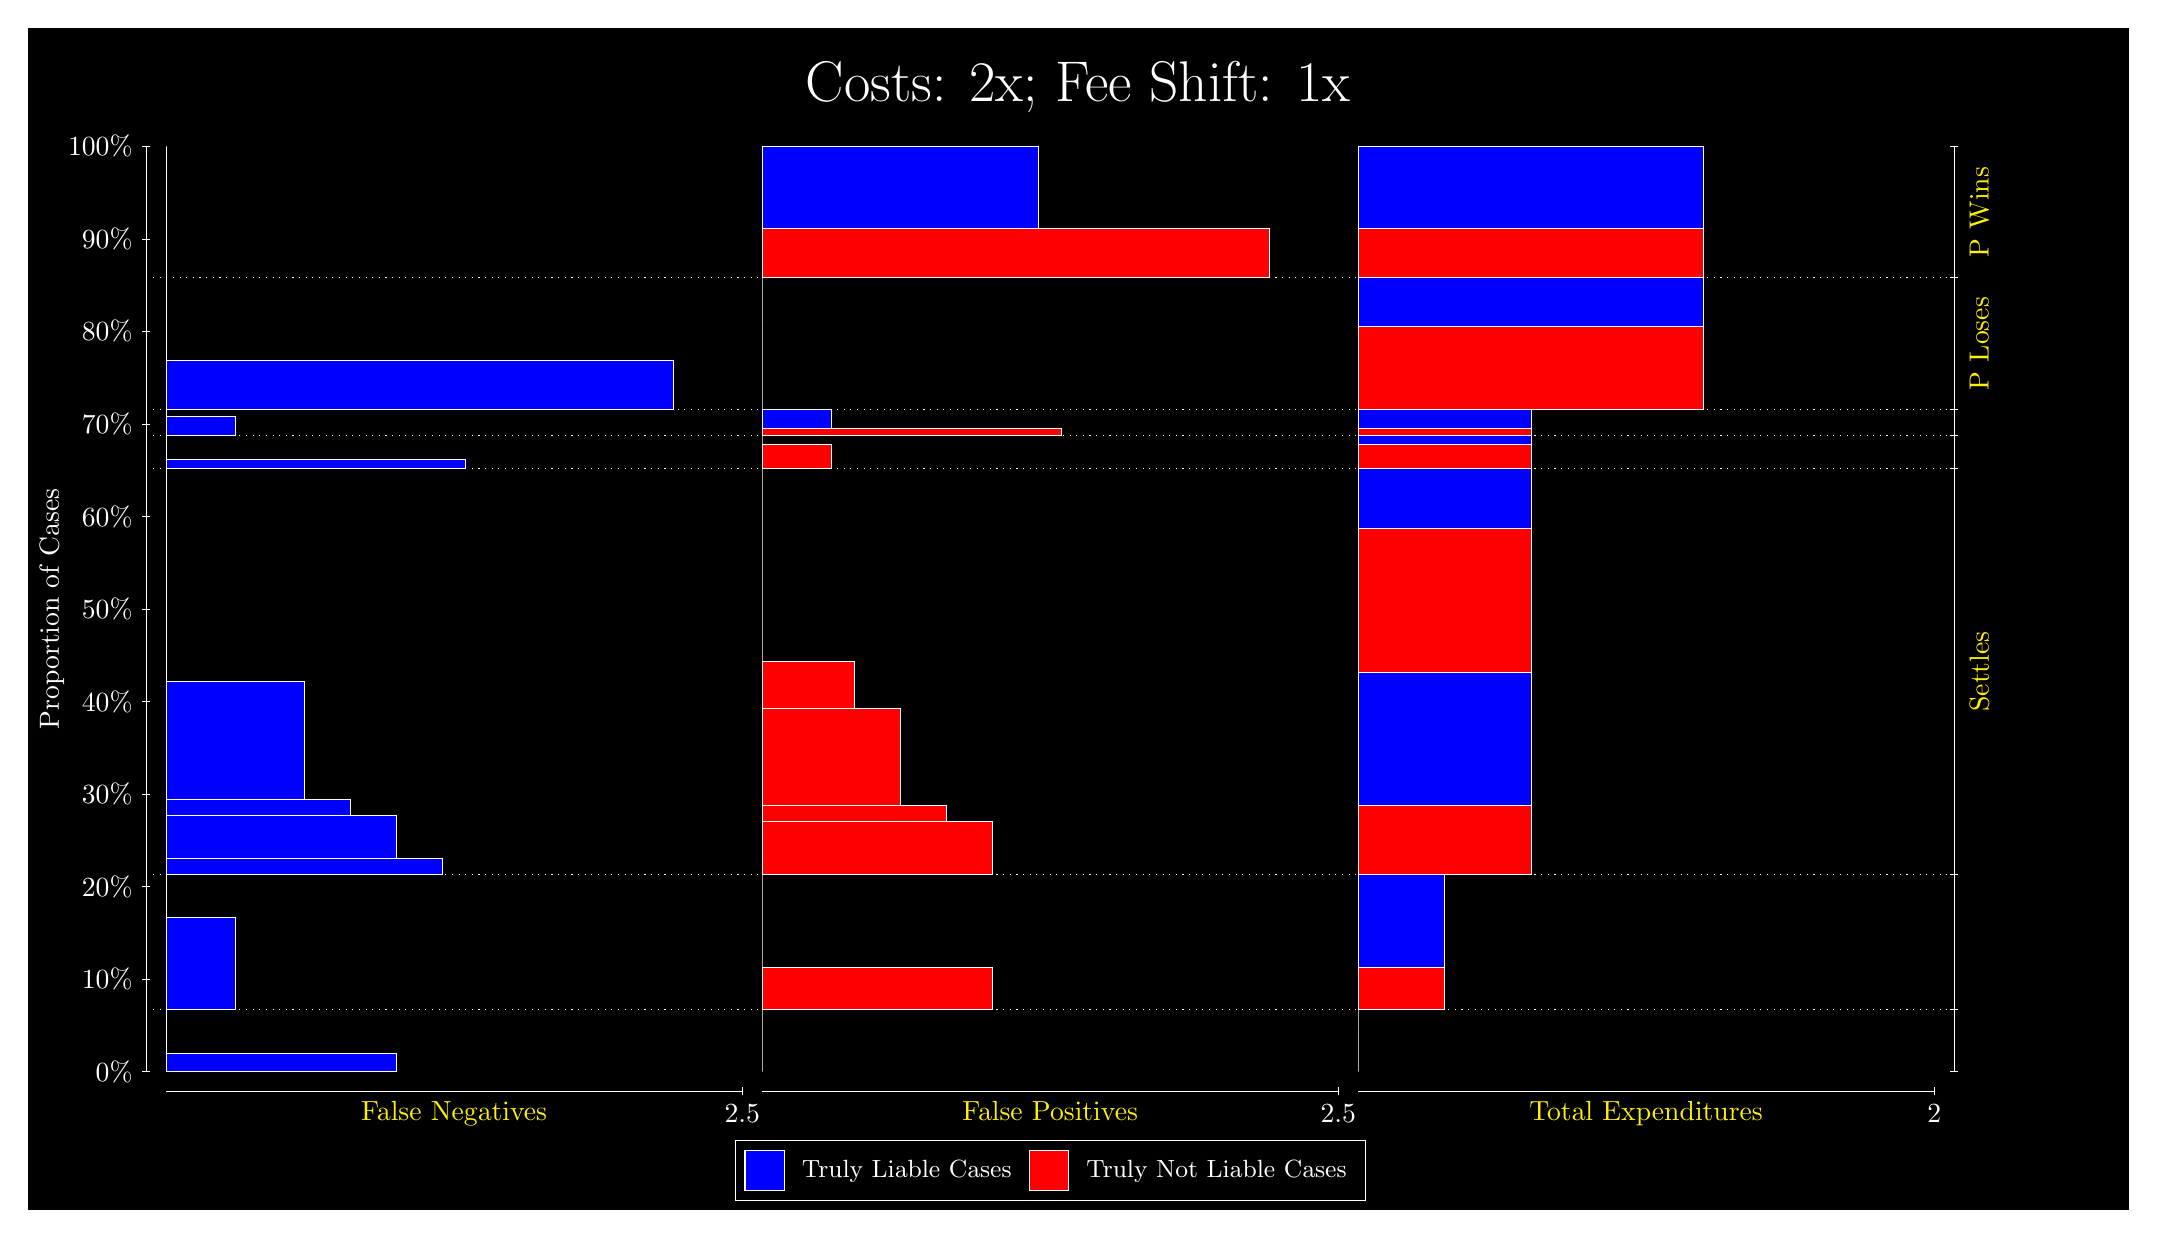
\begin{tikzpicture}
\draw[fill=black] (0,0) rectangle (26.667,15);
\draw[text=white] (0,13.5) rectangle (26.667,15) node[midway] {\huge Costs: 2x; Fee Shift: 1x};
\draw[white, very thin] (1.5,1.75) -- (1.5,13.5);
\node[rotate=90, text=white, anchor=center] at (0.3, 7.625) {Proportion of Cases};
\draw[white, very thin] (1.45,1.75) -- (1.55,1.75);
\node[text=white, anchor=east] at (1.45, 1.75) {0\%};
\draw[white, very thin] (1.45,2.925) -- (1.55,2.925);
\node[text=white, anchor=east] at (1.45, 2.925) {10\%};
\draw[white, very thin] (1.45,4.1) -- (1.55,4.1);
\node[text=white, anchor=east] at (1.45, 4.1) {20\%};
\draw[white, very thin] (1.45,5.275) -- (1.55,5.275);
\node[text=white, anchor=east] at (1.45, 5.275) {30\%};
\draw[white, very thin] (1.45,6.45) -- (1.55,6.45);
\node[text=white, anchor=east] at (1.45, 6.45) {40\%};
\draw[white, very thin] (1.45,7.625) -- (1.55,7.625);
\node[text=white, anchor=east] at (1.45, 7.625) {50\%};
\draw[white, very thin] (1.45,8.8) -- (1.55,8.8);
\node[text=white, anchor=east] at (1.45, 8.8) {60\%};
\draw[white, very thin] (1.45,9.975) -- (1.55,9.975);
\node[text=white, anchor=east] at (1.45, 9.975) {70\%};
\draw[white, very thin] (1.45,11.15) -- (1.55,11.15);
\node[text=white, anchor=east] at (1.45, 11.15) {80\%};
\draw[white, very thin] (1.45,12.325) -- (1.55,12.325);
\node[text=white, anchor=east] at (1.45, 12.325) {90\%};
\draw[white, very thin] (1.45,13.5) -- (1.55,13.5);
\node[text=white, anchor=east] at (1.45, 13.5) {100\%};

\draw[white, very thin] (24.457,1.75) -- (24.457,13.5);
\draw[white, very thin] (24.407,1.75) -- (24.507,1.75);
\node[anchor=west] at (24.407, 1.75) {};
\draw[white, very thin] (24.407,2.5386) -- (24.507,2.5386);
\node[anchor=west] at (24.407, 2.5386) {};
\draw[white, very thin] (24.407,4.2498) -- (24.507,4.2498);
\node[anchor=west] at (24.407, 4.2498) {};
\draw[white, very thin] (24.407,9.4135) -- (24.507,9.4135);
\node[anchor=west] at (24.407, 9.4135) {};
\draw[white, very thin] (24.407,9.8298) -- (24.507,9.8298);
\node[anchor=west] at (24.407, 9.8298) {};
\draw[white, very thin] (24.407,10.158) -- (24.507,10.158);
\node[anchor=west] at (24.407, 10.158) {};
\draw[white, very thin] (24.407,11.832) -- (24.507,11.832);
\node[anchor=west] at (24.407, 11.832) {};
\draw[white, very thin] (24.407,13.5) -- (24.507,13.5);
\node[anchor=west] at (24.407, 13.5) {};

\draw[white, very thin, fill=blue] (1.75,1.75) rectangle (4.6775,1.9772);
\draw[white, very thin, fill=red] (1.75,1.9772) rectangle (1.75,2.5386);
\draw[white, very thin, fill=blue] (1.75,2.5386) rectangle (2.6283,3.7103);
\draw[white, very thin, fill=red] (1.75,3.7103) rectangle (1.75,4.2498);
\draw[white, very thin, fill=blue] (1.75,4.2498) rectangle (5.2631,4.4603);
\draw[white, very thin, fill=blue] (1.75,4.4603) rectangle (4.6775,5.0103);
\draw[white, very thin, fill=blue] (1.75,5.0103) rectangle (4.092,5.2116);
\draw[white, very thin, fill=blue] (1.75,5.2116) rectangle (3.5065,6.7072);
\draw[white, very thin, fill=red] (1.75,6.7072) rectangle (1.75,9.4135);
\draw[white, very thin, fill=blue] (1.75,9.4135) rectangle (5.5558,9.5296);
\draw[white, very thin, fill=red] (1.75,9.5296) rectangle (1.75,9.8298);
\draw[white, very thin, fill=blue] (1.75,9.8298) rectangle (2.6283,10.066);
\draw[white, very thin, fill=red] (1.75,10.066) rectangle (1.75,10.158);
\draw[white, very thin, fill=blue] (1.75,10.158) rectangle (8.1906,10.777);
\draw[white, very thin, fill=red] (1.75,10.777) rectangle (1.75,11.832);
\draw[white, very thin, fill=red] (1.75,11.832) rectangle (1.75,12.453);
\draw[white, very thin, fill=blue] (1.75,12.453) rectangle (1.75,13.5);
\draw[white, very thin, fill=red] (9.3189,1.75) rectangle (9.3189,2.3114);
\draw[white, very thin, fill=blue] (9.3189,2.3114) rectangle (9.3189,2.5386);
\draw[white, very thin, fill=red] (9.3189,2.5386) rectangle (12.246,3.0781);
\draw[white, very thin, fill=blue] (9.3189,3.0781) rectangle (9.3189,4.2498);
\draw[white, very thin, fill=red] (9.3189,4.2498) rectangle (12.246,4.9268);
\draw[white, very thin, fill=red] (9.3189,4.9268) rectangle (11.661,5.128);
\draw[white, very thin, fill=red] (9.3189,5.128) rectangle (11.075,6.359);
\draw[white, very thin, fill=red] (9.3189,6.359) rectangle (10.49,6.9561);
\draw[white, very thin, fill=blue] (9.3189,6.9561) rectangle (9.3189,9.4135);
\draw[white, very thin, fill=red] (9.3189,9.4135) rectangle (10.197,9.7137);
\draw[white, very thin, fill=blue] (9.3189,9.7137) rectangle (9.3189,9.8298);
\draw[white, very thin, fill=red] (9.3189,9.8298) rectangle (13.125,9.9216);
\draw[white, very thin, fill=blue] (9.3189,9.9216) rectangle (10.197,10.158);
\draw[white, very thin, fill=red] (9.3189,10.158) rectangle (9.3189,11.213);
\draw[white, very thin, fill=blue] (9.3189,11.213) rectangle (9.3189,11.832);
\draw[white, very thin, fill=red] (9.3189,11.832) rectangle (15.759,12.453);
\draw[white, very thin, fill=blue] (9.3189,12.453) rectangle (12.832,13.5);
\draw[white, very thin, fill=red] (16.888,1.75) rectangle (16.888,2.3114);
\draw[white, very thin, fill=blue] (16.888,2.3114) rectangle (16.888,2.5386);
\draw[white, very thin, fill=red] (16.888,2.5386) rectangle (17.986,3.0781);
\draw[white, very thin, fill=blue] (16.888,3.0781) rectangle (17.986,4.2498);
\draw[white, very thin, fill=red] (16.888,4.2498) rectangle (19.083,5.128);
\draw[white, very thin, fill=blue] (16.888,5.128) rectangle (19.083,6.825);
\draw[white, very thin, fill=red] (16.888,6.825) rectangle (19.083,8.653);
\draw[white, very thin, fill=blue] (16.888,8.653) rectangle (19.083,9.4135);
\draw[white, very thin, fill=red] (16.888,9.4135) rectangle (19.083,9.7137);
\draw[white, very thin, fill=blue] (16.888,9.7137) rectangle (19.083,9.8298);
\draw[white, very thin, fill=red] (16.888,9.8298) rectangle (19.083,9.9216);
\draw[white, very thin, fill=blue] (16.888,9.9216) rectangle (19.083,10.158);
\draw[white, very thin, fill=red] (16.888,10.158) rectangle (21.279,11.213);
\draw[white, very thin, fill=blue] (16.888,11.213) rectangle (21.279,11.832);
\draw[white, very thin, fill=red] (16.888,11.832) rectangle (21.279,12.453);
\draw[white, very thin, fill=blue] (16.888,12.453) rectangle (21.279,13.5);
\draw[white, dotted] (1.5,2.5386) -- (24.457,2.5386);
\draw[white, dotted] (1.5,4.2498) -- (24.457,4.2498);
\draw[white, dotted] (1.5,9.4135) -- (24.457,9.4135);
\draw[white, dotted] (1.5,9.8298) -- (24.457,9.8298);
\draw[white, dotted] (1.5,10.158) -- (24.457,10.158);
\draw[white, dotted] (1.5,11.832) -- (24.457,11.832);
\draw[white, very thin] (1.75,1.5) -- (9.0689,1.5);
\node[text=yellow, anchor=north] at (5.4094, 1.5) {False Negatives};
\draw[white, very thin] (9.0689,1.45) -- (9.0689,1.55);
\node[text=white, anchor=north] at (9.0689, 1.45) {2.5};

\draw[white, very thin] (9.3189,1.5) -- (16.638,1.5);
\node[text=yellow, anchor=north] at (12.978, 1.5) {False Positives};
\draw[white, very thin] (16.638,1.45) -- (16.638,1.55);
\node[text=white, anchor=north] at (16.638, 1.45) {2.5};

\draw[white, very thin] (16.888,1.5) -- (24.207,1.5);
\node[text=yellow, anchor=north] at (20.547, 1.5) {Total Expenditures};
\draw[white, very thin] (24.207,1.45) -- (24.207,1.55);
\node[text=white, anchor=north] at (24.207, 1.45) {2};



\node[text=yellow, centered, rotate=90] at (24.777, 6.8316) {Settles};


\node[text=yellow, centered, rotate=90] at (24.777, 10.995) {P Loses};
\node[text=yellow, centered, rotate=90] at (24.777, 12.666) {P Wins};

\draw (12.978300999999998,1.5) node[draw=none] (baseCoordinate) {};
\begin{scope}[align=center]
        \matrix[scale=0.5, draw=white, below=0.5cm of baseCoordinate, nodes={draw}, column sep=0.1cm]{
            \node[rectangle, draw, minimum width=0.5cm, minimum height=0.5cm, fill=blue] {}; &
            \node[draw=none, font=\small, text=white] (B) {Truly Liable Cases}; &
            \node[rectangle, draw, minimum width=0.5cm, minimum height=0.5cm, fill=red] {}; &
            \node[draw=none, font=\small, text=white] (B) {Truly Not Liable Cases}; \\
            };
\end{scope}

\end{tikzpicture}
\end{document}